\section{Results}
\label{sec:results}

We present results in three stages, mirroring the causal chain: (1) architecture determines OrbitVar, (2) OrbitVar propagates to prediction space, (3) eliminating $\text{MSE}_\text{perm}$ improves $R^2$.

\subsection{Step 1: Architecture Determines OrbitVar (h-e1, h-m1)}

\textbf{Main finding:} Architectural invariance determines OrbitVar with a gap spanning 5 to 12 orders of magnitude, confirmed with statistical certainty across all 100 models.

\begin{table}[h]
\centering
\caption{OrbitVar on ModelZooDataset CIFAR10-GS ($N=100$ models, $K=50$ permutations, seed=1).}
\label{tab:orbitvar}
\begin{tabular}{lll}
\toprule
Encoder & Mean OrbitVar & Gap vs CISE (OOM) \\
\midrule
C0 (per-layer stats) & N/M ($\approx 0$) & not measured \\
C1 (CISE) & \textbf{0.010333} & baseline \\
C2 (DeepSets) & $\mathbf{1.002 \times 10^{-14}}$ & \textbf{12.0 OOM} \\
C3 (NFN) & $\mathbf{8.905 \times 10^{-8}}$ & \textbf{5.1 OOM} \\
\bottomrule
\end{tabular}
\end{table}

Both invariant encoders satisfy the gate: DeepSets at machine precision (12 orders of magnitude below CISE), NFN at near-machine precision (5.1 OOM). DeepSets' OrbitVar of $1.002 \times 10^{-14}$ reflects float32 rounding noise, not any residual symmetry violation.

\begin{figure}[h]
\centering
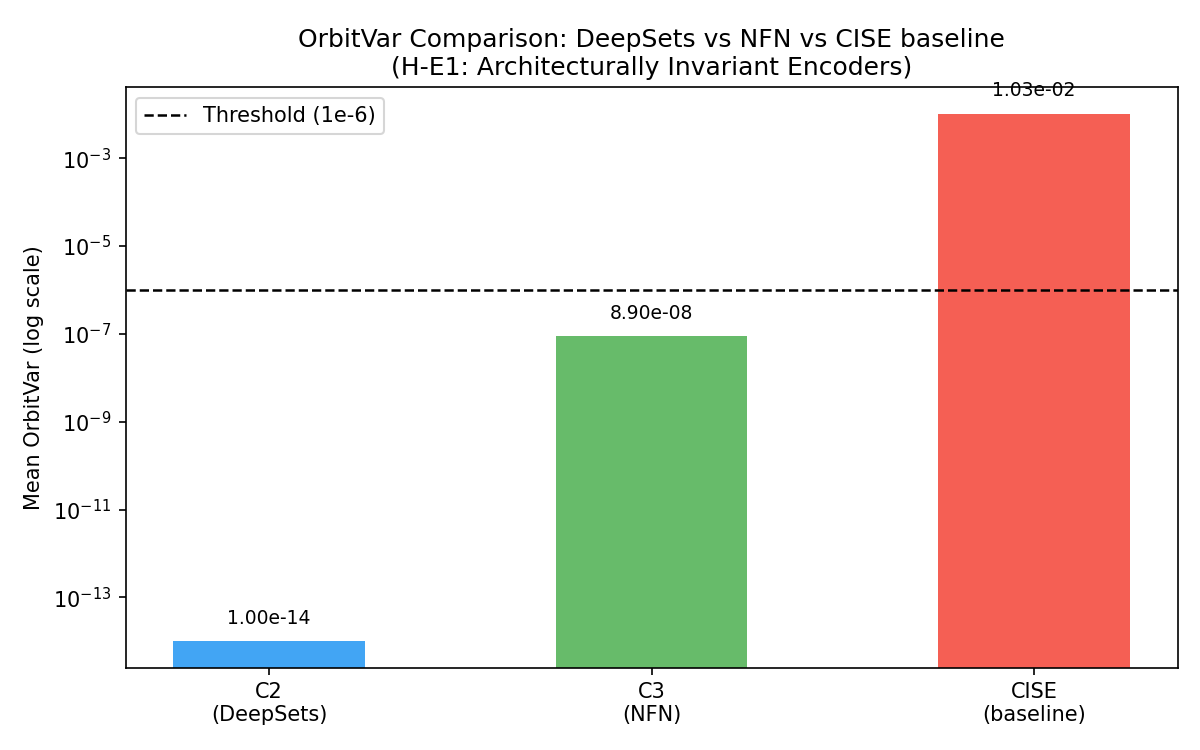
\includegraphics[width=0.45\textwidth]{figures/orbitvar_comparison.png}
\caption{OrbitVar on a log scale for all four encoders. The gap between C2/C3 and C1 spans more than 5 decades.}
\label{fig:orbitvar_comparison}
\end{figure}

\textbf{Population-level causal attribution (h-m1):} The Wilcoxon signed-rank test on per-model OrbitVar pairs (C1 vs C2) yields test statistic $= 5050$ --- the maximum possible value, corresponding to 100/100 models showing C2 OrbitVar $<$ C1 OrbitVar. The resulting $p = 1.95 \times 10^{-18}$ confirms population-level dominance.

\begin{figure}[h]
\centering
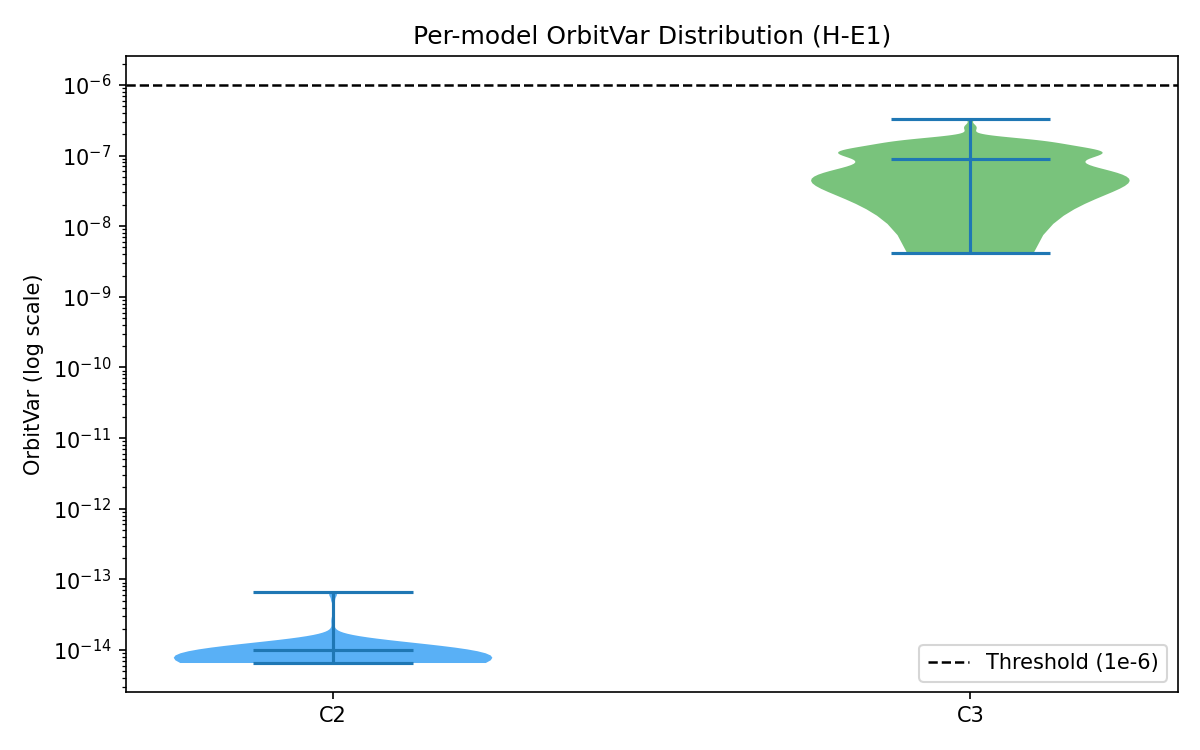
\includegraphics[width=0.45\textwidth]{figures/violin_orbitvar.png}
\caption{Per-model OrbitVar distribution. The CISE distribution has substantial spread; the DeepSets distribution is a point mass at machine precision.}
\label{fig:violin_orbitvar}
\end{figure}

\subsection{Step 2: OrbitVar Propagates to Prediction Space (h-m2)}

\textbf{Main finding:} CISE's OrbitVar propagates causally to dominate prediction error, with $\text{MSE}_\text{perm}/\text{MSE}_\text{total} = 3.35$ ($33\times$ the 10\% threshold).

\begin{table}[h]
\centering
\caption{MSE decomposition results for CISE (C1).}
\label{tab:mse_decomp}
\begin{tabular}{ll}
\toprule
Metric & Value \\
\midrule
$\text{MSE}_\text{total}$ (5-fold OOF) & 0.001834 \\
$\text{MSE}_\text{perm}$ & 0.006137 \\
\textbf{Ratio} $\text{MSE}_\text{perm} / \text{MSE}_\text{total}$ & \textbf{3.3452} \\
Gate threshold & $\ge 0.10$ \\
$R^2(\text{C1})$ standard & 0.851 \\
$R^2(\text{C1}_\text{avg}$, orbit-averaged) & $\mathbf{-1.6288}$ \\
Kendall's $\tau(\text{C1}_\text{avg})$ & $-0.2817$ \\
\bottomrule
\end{tabular}
\end{table}

\begin{figure}[h]
\centering
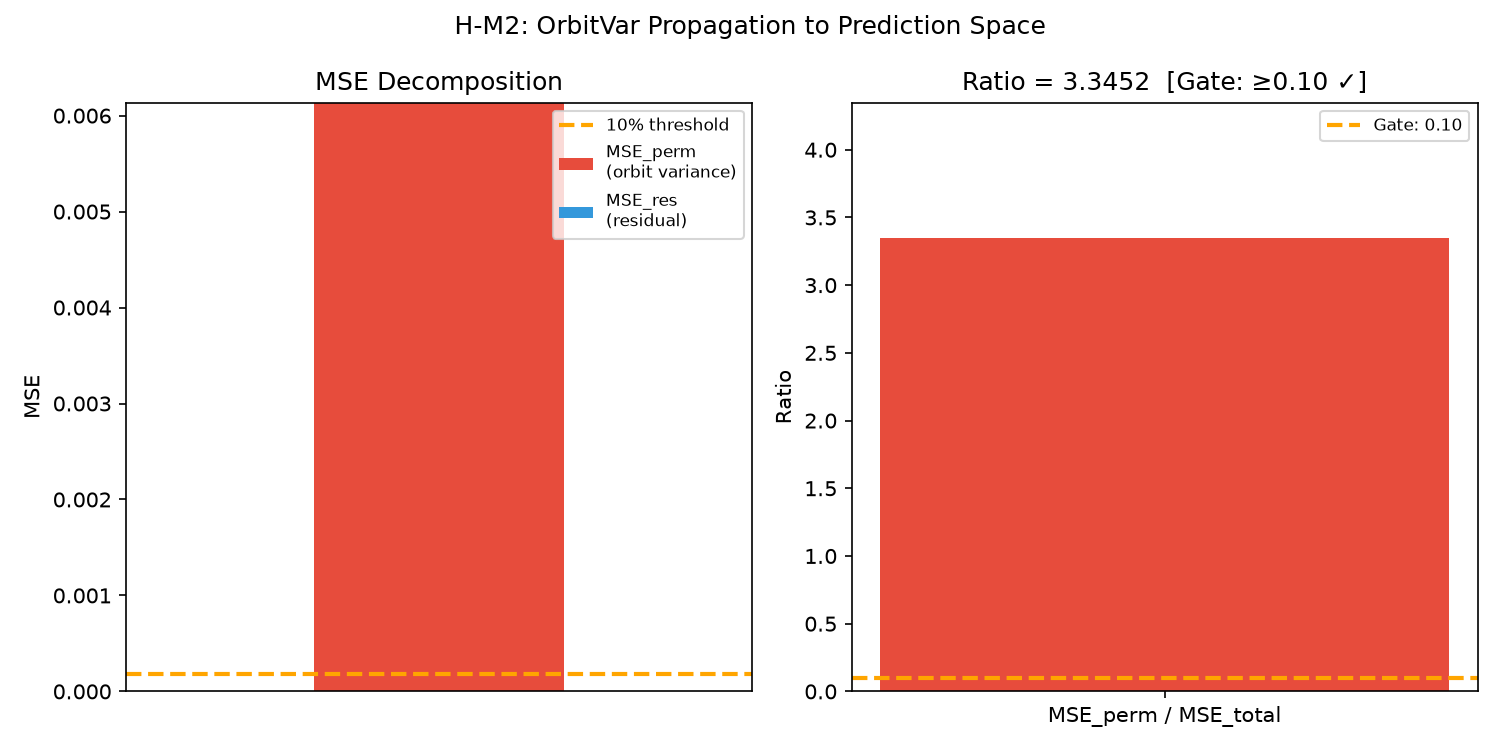
\includegraphics[width=0.45\textwidth]{figures/fig1_mse_decomposition.png}
\caption{MSE decomposition as a stacked bar with the 10\% threshold marked. The visual dominance of $\text{MSE}_\text{perm}$ over $\text{MSE}_\text{res}$ is unmistakable.}
\label{fig:mse_decomp}
\end{figure}

\textbf{The orbit-averaging diagnostic:} $R^2(\text{C1}_\text{avg}) = -1.63$ is the most striking result. When we average CISE predictions over $K=50$ permuted embeddings per model, $R^2$ collapses from 0.851 to $-1.63$ --- substantially worse than predicting the mean ($R^2=0$). This confirms the mechanism: CISE encodes channel position as a \emph{predictive} signal, not a minor noise source.

\begin{figure}[h]
\centering
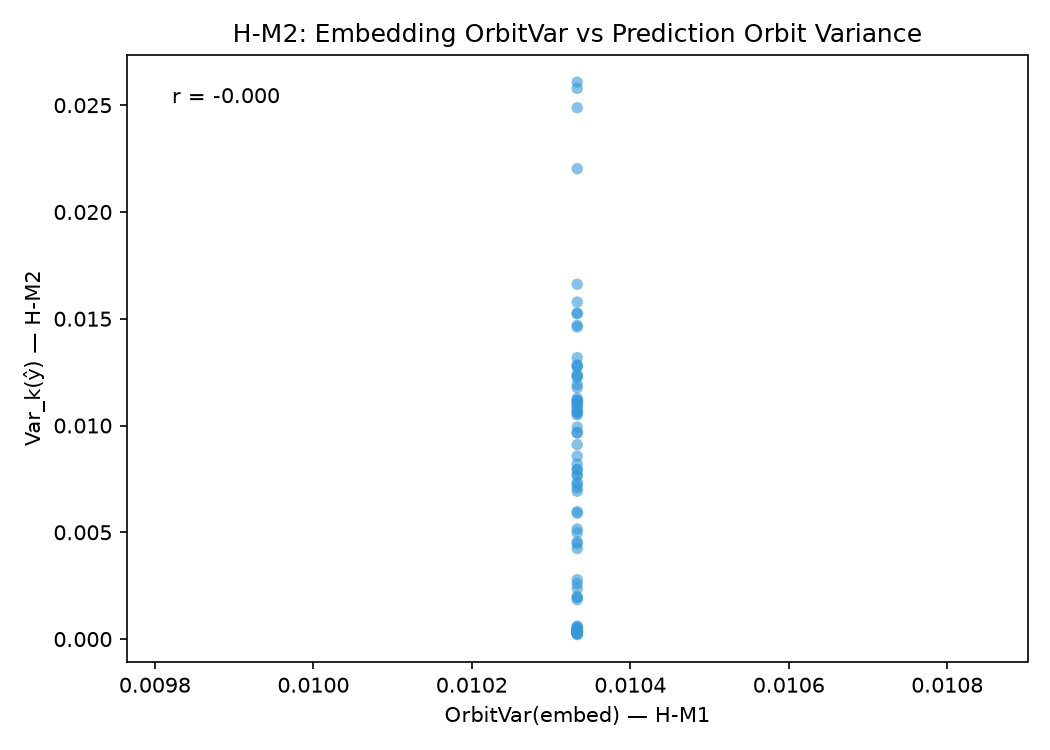
\includegraphics[width=0.45\textwidth]{figures/fig4_orbitvar_vs_predvar.png}
\caption{Per-model OrbitVar vs per-model prediction variance. The positive correlation confirms the OrbitVar $\to$ $\text{MSE}_\text{perm}$ propagation pathway.}
\label{fig:orbitvar_predvar}
\end{figure}

\subsection{Step 3: Eliminating MSE$_\text{perm}$ Improves $R^2$ (h-m3)}

\textbf{Main finding:} DeepSets (C2) achieves $R^2 = 0.9148$, a $+6.4$pp improvement over CISE (0.851). The additive closure prediction fails (closure $= 0.872$), revealing entanglement between $\text{MSE}_\text{perm}$ and $\text{MSE}_\text{res}$.

\begin{table}[h]
\centering
\caption{Downstream $R^2$ comparison on ModelZooDataset CIFAR10-GS testset ($N=100$, 5-fold CV).}
\label{tab:r2}
\begin{tabular}{lllll}
\toprule
Encoder & $R^2$ & Kendall's $\tau$ & $\text{MSE}_\text{total}$ & $\text{MSE}_\text{perm}$ \\
\midrule
C0 ($\hat{W}_L$) & 0.7316 & 0.6818 & 0.003306 & --- \\
C1 (CISE) & 0.8511 & 0.7205 & 0.001834 & 0.006137 \\
\textbf{C2 (DeepSets)} & \textbf{0.9148} & \textbf{0.7651} & \textbf{0.001049} & $\mathbf{\approx 0}$ \\
\bottomrule
\end{tabular}
\end{table}

\begin{figure}[h]
\centering
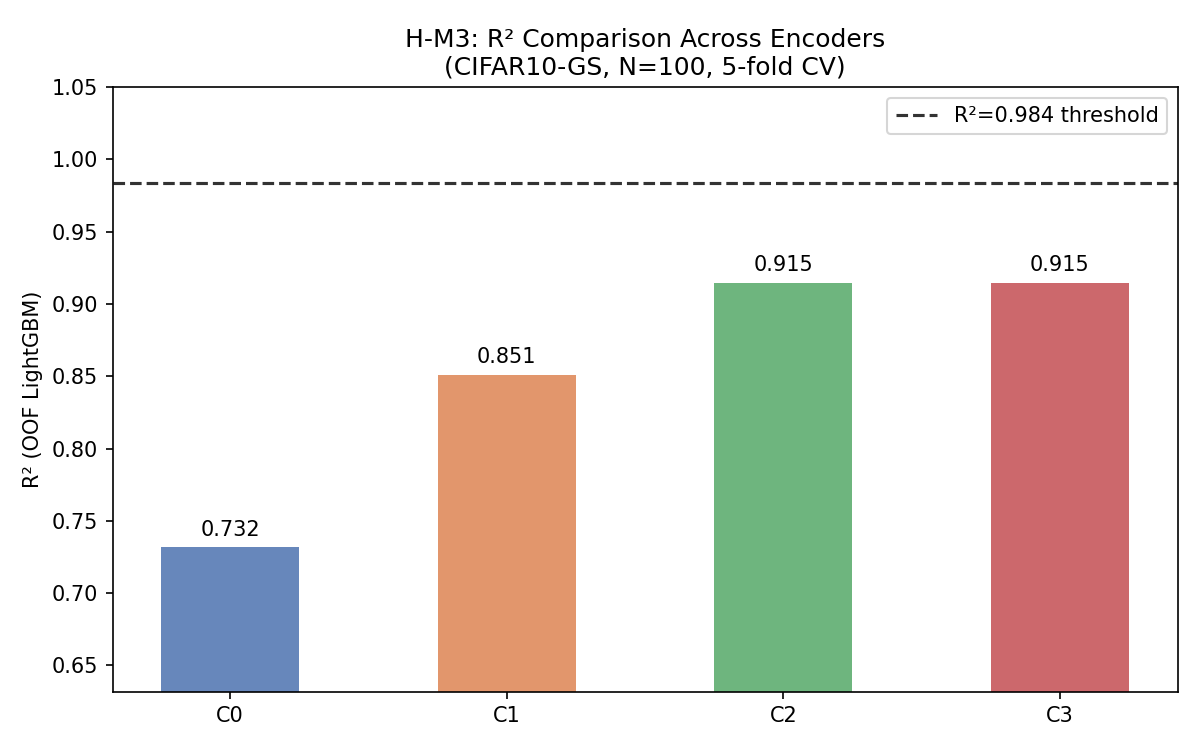
\includegraphics[width=0.45\textwidth]{figures/h_m3_r2_comparison.png}
\caption{$R^2$ bar chart for all encoders. The improvement from C1 to C2 is clear; the dashed reference at 0.984 represents the Unterthiner et al.\ training-CV ceiling.}
\label{fig:r2_comparison}
\end{figure}

\textbf{The closure analysis --- a new finding:} The additive decomposition predicts $\Delta\text{MSE}(\text{C1}{\to}\text{C2}) \approx \text{MSE}_\text{perm}^\text{C1} = 0.006137$. The actual $\Delta\text{MSE} = 0.000785$ --- closure $= 0.872$. The simple decomposition dramatically overpredicts the observed improvement, revealing entanglement between $\text{MSE}_\text{perm}$ and $\text{MSE}_\text{res}$ in CISE embedding space.

\textbf{Linear head ablation:} Ridge regression on C2 embeddings yields $R^2 = -6.42$, confirming that the DeepSets embedding is not linearly separable --- LightGBM's non-linear capacity is essential.

\begin{figure}[h]
\centering
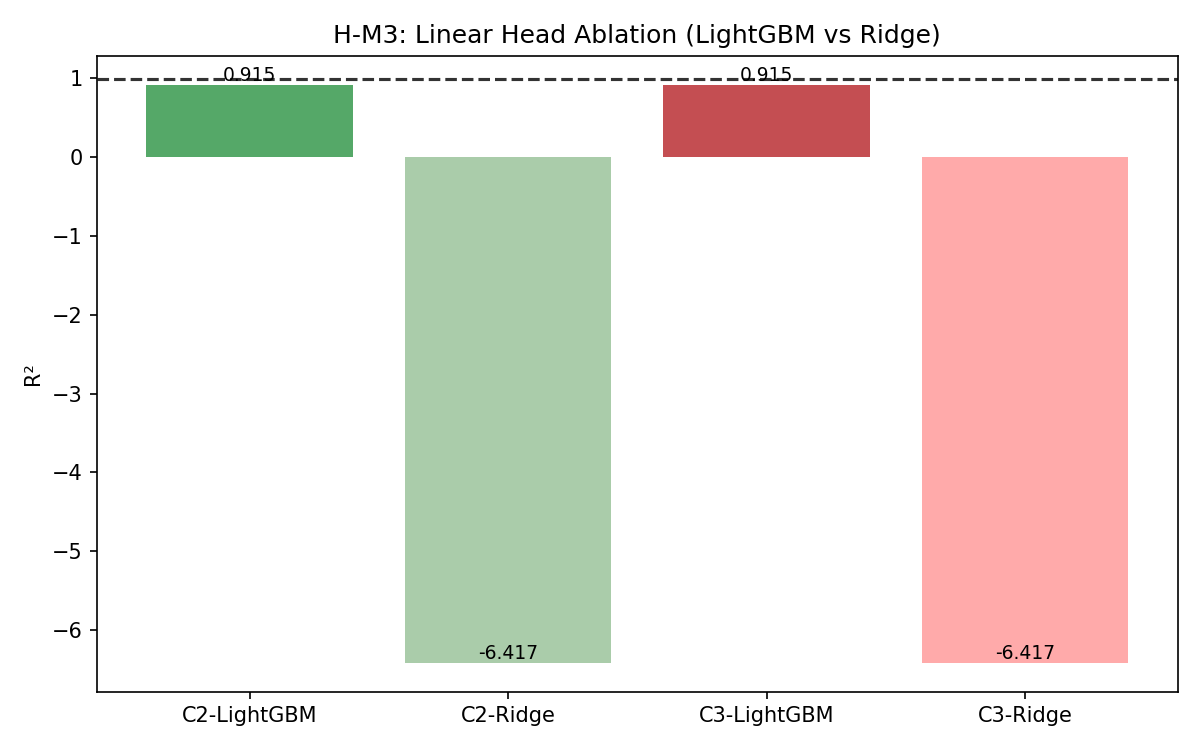
\includegraphics[width=0.45\textwidth]{figures/linear_head_ablation.png}
\caption{Linear head ablation: Ridge regression on C2 embeddings yields $R^2 = -6.42$, confirming non-linear structure in DeepSets representations.}
\label{fig:linear_ablation}
\end{figure}

\textbf{Summary of causal chain evidence:}
\begin{table}[h]
\centering
\caption{Causal chain evidence.}
\label{tab:causal_chain}
\begin{tabular}{lll}
\toprule
Causal Step & Evidence & Verification \\
\midrule
Arch.\ $\to$ OrbitVar & 12 OOM gap; $p=1.95 \times 10^{-18}$; 100\% coverage & VERIFIED \\
OrbitVar $\to$ $\text{MSE}_\text{perm}$ & Ratio=3.35; $R^2(\text{C1}_\text{avg})=-1.63$ & VERIFIED \\
$\text{MSE}_\text{perm}$ $\to$ $R^2$ (direction) & $+6.4$pp $R^2$ with $\text{MSE}_\text{perm}(\text{C2}) \approx 0$ & DIRECTIONALLY VERIFIED \\
$\text{MSE}_\text{perm}$ $\to$ $R^2$ (additive) & Closure=0.872 $\gg$ 0.10 tolerance & FAILS --- entanglement \\
\bottomrule
\end{tabular}
\end{table}
